\entete{FOD}{12 F�vrier 2012}

\section{Alg\`ebre relationnelle et SQL (10 points)}

Voici une partie de la base de donn\'ees utilis\'ee pour g\'erer des {\oe}uvres
dans un mus\'ee:
 
\smallskip

\texttt{\textbf{Oeuvre}(id\_oeuvre, nom, id\_auteur, valeur\_assurance, date\_acquisition, lieu\_exposition, description)}\\ 
\texttt{\textbf{Auteur}(id\_auteur, nom, prenom, date\_naissance, date\_deces)}\\ 
\texttt{\textbf{Expert}(id\_expert, nom, prenom, domaine\_expertise)}\\
\texttt{\textbf{Expertise}(id\_oeuvre, id\_expert, date\_evaluation, valeur)}\\
\smallskip


Informations suppl\'ementaires : Des experts expertisent des {\oe}uvres.
Plusieurs experts peuvent expertiser une m\^eme {\oe}uvre. 
\`A partir de ces expertises, une valeur est d\'eduite pour l'assurance de l'{\oe}uvre.

\begin{enumerate}

\item Pour chaque table, identifier les cl\'es primaires et les cl\'es
  \'etrang\`eres. (1 point)
\begin{correction}\\
\begin{itemize}
\item Cl\'es primaires\\
    Table \texttt{Oeuvre : id\_oeuvre}\\
    Table \texttt{Auteur : id\_auteur}\\
    Table \texttt{Expert : id\_expert}\\ 
    Table \texttt{Expertise : (id\_oeuvre, id\_expert)}\\
    ou \'eventuellement (selon interpr\'etation) \texttt{Expertise : (id\_oeuvre, id\_expert, date\_evaluation)}
\item Cl\'es \'etrang\`eres :\\
  \texttt{Oeuvre[id\_auteur] $\subseteq$ Auteur[id\_auteur]}\\
  \texttt{Expertise[id\_oeuvre] $\subseteq$ Oeuvre[id\_oeuvre]}\\
  \texttt{Expertise[id\_expert] $\subseteq$ Expert[id\_expert]}\\
\end{itemize}
\end{correction}

\item Donner des commandes SQL permettant de cr\'eer les tables
\texttt{\textbf{Oeuvre}} et \texttt{\textbf{Auteur}}. (1 point) 
  
\begin{correction}
  \begin{lstlisting}
  CREATE TABLE Auteur (
  id_auteur INTEGER NOT NULL,
  nom VARCHAR2(20),
  prenom VARCHAR2(20),
  date_naissance DATE,
  date_deces DATE,
  CONSTRAINT Auteur_PK PRIMARY KEY (id_auteur)
  );

  CREATE TABLE Oeuvre (
  id_oeuvre INTEGER NOT NULL,
  nom VARCHAR2(40),
  id_auteur INTEGER,
  valeur_assurance INTEGER,
  date_acquisition DATE,
  lieu_exposition VARCHAR2(30),
  description VARCHAR2(60),
  CONSTRAINT Oeuvre_PK PRIMARY KEY (id_oeuvre)
  CONSTRAINT Oeuvre_id_auteurKF FOREIGN KEY (id_auteur) REFERENCES Auteur (id_auteur) );
  \end{lstlisting}

\end{correction}

\item Donner les identifiants des {\oe}uvres dont la valeur assurance est comprise entre
  10\,000 et 50\,000 euros. Alg\`ebre et SQL (1 point) 
\begin{correction}\\
  Alg\`ebre:\\ $\pi_{id\_oeuvre}(\sigma_{valeur\_assurance \ge 10000 \land valeur\_assurance \le
  50000}(Oeuvre))$\\ 
  SQL: 
   \begin{lstlisting}
    SELECT id_oeuvre FROM Oeuvre
    WHERE valeur_assurance >= 10000 AND valeur_assurance <= 50000;
    \end{lstlisting}
\end{correction}

\item Donner les noms et pr\'enoms des experts ayant expertis\'e l'{\oe}uvre dont
  l'identifiant est 345801. Alg\`ebre et SQL. (2 points) 
  
\begin{correction}\\ Alg\`ebre: Jointure sur l'id de l'expert\\
    $\pi_{nom,prenom}(Expert \Join \sigma_{id\_oeuvre=345801}(Expertise))$\\ 
    SQL:
 \begin{lstlisting}
    SELECT e.nom, e.prenom FROM Expert e, Expertise v
    WHERE e.id_expert = v.id_expert AND id_oeuvre=345801;
 \end{lstlisting}
\end{correction}

\item Donner, pour chaque auteur (nom et pr\'enom), la valeur
  d'assurance (cumul\'ee) de ses {\oe}uvres. SQL seulement (1 point) 
\begin{correction}
 \begin{lstlisting}
  SELECT a.nom, a.prenom, sum(valeur_assurance)
  FROM Auteur a, Oeuvre o
  WHERE o.id_auteur=a.id_auteur
  GROUP BY a.id_auteur, a.nom, a.prenom;
 \end{lstlisting}
\end{correction}
  
\item Donner les identifiants des {\oe}uvres de la \textit{salle 1}
  (\textit{salle 1} est un lieu d'exposition) ayant \'et\'e expertis\'ees par au
  moins deux experts. Alg\`ebre
  et SQL. (3 points) 
  
\begin{correction}\\ 
  
  Alg\`ebre (une solution parmi d'autres):\\ 
 $R_1$ (identifiants des {\oe}uvres de la salle 1)\\
 $\pi_{id\_oeuvre}(\sigma_{lieu\_exposition='salle 1'}(Oeuvre))$\\
 
 $R_2$ (identifiants des {\oe}uvres expertis\'ees par au moins deux experts):\\
 $\pi_{id\_oeuvre}\biggl(\sigma_{id\_oeuvre=id\_oeuvre2 \atop
 \wedge id\_expert \neq id\_expert2}\Bigl(Expertise \times \rho_{id\_oeuvre \rightarrow
 id\_oeuvre2, \atop id\_expert \rightarrow
 id\_expert2}(Expertise)\Bigr)\biggr)$\\
  ou une autre solution pour $R_2$ :\\
$\pi_{id\_oeuvre}\biggl(\sigma_{id\_expert \neq id\_expert2}\Bigl(Expertise \Join \rho_{id\_expert
\rightarrow id\_expert2, valeur \rightarrow valeur2, \atop date\_evaluation \rightarrow
 date\_evaluation2}(Expertise)\Bigr)\biggr)$\\
 
 $R_3$ (solution):\\
 $R_1 \cap R_2$

   SQL (une solution parmi d'autres):
   \begin{lstlisting}
   SELECT o.id_oeuvre
   FROM Expertise e1, Expertise e2, Oeuvre o
   WHERE e1.id_oeuvre=e2.id_oeuvre AND e1.id_expert <> e2.id_expert AND
   e1.id_oeuvre = o.id_oeuvre AND o.lieu_exposition='salle 1';
   \end{lstlisting}
   ou 
   \begin{lstlisting}
   SELECT o.id_oeuvre
   FROM Expertise e, Oeuvre o
   WHERE e.id_oeuvre = o.id_oeuvre AND lieu_exposition='salle 1'
   GROUP BY id_oeuvre
   HAVING count(e.id_expert) >= 2;
   \end{lstlisting}
	
	Nous avons consid�r� qu'un m�me expert pouvait expertiser plusieurs fois une m�me oeuvre, la cl� primaire de la table \texttt{Expertise} �tant donc \texttt{(id\_oeuvre, id\_expert, date\_evaluation)}.

\end{correction}

  
\item Donner les identifiants des experts ayant expertis\'e toutes les
  {\oe}uvres de Edward HOPPER.
  Alg\`ebre seulement. (1 point) 
\begin{correction}\\
  $R_1$ (les identifiants des {\oe}uvres de Edward Hopper) :\\
  $\pi_{id\_oeuvre}(Oeuvre \Join (\rho_{nom \rightarrow
  nom\_auteur}(\sigma_{nom='Hopper' \wedge prenom='Edward'} (Auteur))))$.
  Attention ici au renommage de l'attribut $nom$ si on utilise une jointure
  naturelle. \\ 
  
  $R_2$ (la correction):\\
  $(\pi_{id\_expert,id\_oeuvre}(Expertise)) \div R_1$
\end{correction}
  
\end{enumerate}
 
 
\section{Indexation (3 points)}

On s'int\'eresse aux designers industriels et on ins\`ere successivement les enregistrements suivants dans la table Auteur, selon cet ordre :

\begin{center}
\begin{small}
\begin{tabular}{ccccc}
id\_auteur & \textbf{nom} & prenom & date\_naissance & date\_deces\\
1 & Saarinen & Eero & 1910 & 1961\\
2 & Jacobsen & Arne & 1902 & 1971\\
3 & Le Corbusier & NULL & 1887 & 1965\\
4 & Eames & Charles & 1907 & 1978\\
5 & Bertoia & Harry & 1915 & 1978\\
6 & Panton & Verner & 1926 & 1998\\
7 & Jouin & Patrick & 1967 & NULL\\
8 & Starck & Philippe & 1949 & NULL\\
\end{tabular}

\begin{tabular}{ccccc}
id\_auteur & \textbf{nom} & prenom & date\_naissance & date\_deces\\
9 & Noguchi & Isamu & 1904 & 1988\\
10 & Nelson & George & 1908 & 1986\\
11 & Perriand & Charlotte & 1903 & 1999\\
12 & Prouv\'e & Jean & 1901 & 1984\\
13 & Aalto & Alvar & 1898 & 1976\\
14 & Gray & Eileen & 1878 & 1976\\
15 & Breuer & Marcel & 1902 & 1981\\
16 & Tallon & Roger & 1929 & 2011
\end{tabular}

\end{small}
\end{center}

On met en place un index sur l'attribut \textbf{nom} de cette table. 

\begin{enumerate}
\item Construire l'arbre B+ d'ordre 2 correspondant \`a cet ensemble d'articles, en respectant l'ordre d'arriv\'ee. Donner les \'etapes de construction interm\'ediaires importantes (celles qui produisent un changement de la structure de l'arbre) et distinguer sur les sch\'emas les n{\oe}uds de natures diff\'erentes (n{\oe}uds contenant des cl\'es vs. ceux contenant les enregistrements complets ou autre chose). (1,5 point)

\begin{correction}

La figure \ref{fi:sol_Bp} donne l'arbre B+ d'ordre 2 obtenu. Ici les n{\oe}uds internes (en italique) contiennent les cl\'es des enregistrements, alors que les n{\oe}uds feuilles (en gras) contiennent les enregistrements complets, ou bien leurs cl\'es plus les pointeurs vers ces enregistrements sur disque.

\begin{figure}[htbp]
\begin{center}
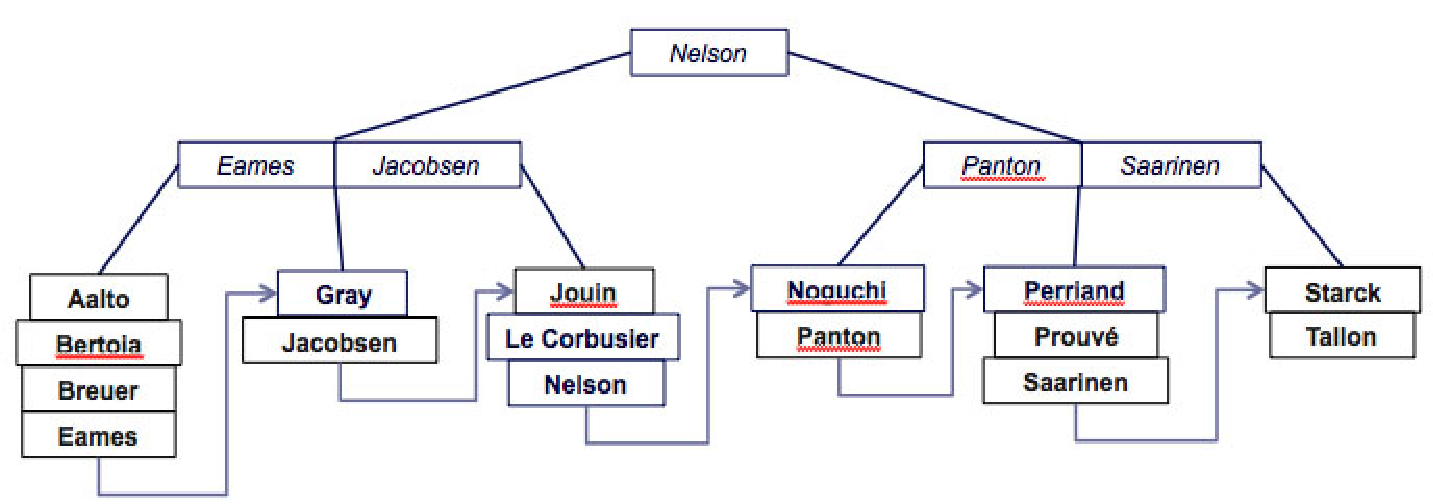
\epsfig{file=Fig/2012-02_bptree, width=15cm}
\end{center}
\caption{Arbre B+ d'ordre 2.}
\label{fi:sol_Bp}
\end{figure}

\end{correction}

\item On recherche le pr\'enom des designers dont l'initiale du nom se trouve entre 'H' et 'N'. Combien de pages disque doivent \^etre charg\'ees pour r\'epondre \`a cette requ\^ete en utilisant l'arbre B+ ? Justifier. (1 point)

\begin{correction}

Il s'agit ici d'une requ\^ete par intervalle, facilement r\'ealisable avec un arbre B+. On commence par faire une recherche du premier enregistrement dont l'initiale du nom est \'egale ou imm\'ediatement sup\'erieure \`a 'H'. On charge le n{\oe}ud racine 'Nelson' puis son fils gauche puisque 'H' pr\'ec\`ede 'N'. 'H' se situant entre 'Eames' et 'Jacobsen', on lit ensuite le n{\oe}ud feuille relatif aux enregistrements 'Gray' et 'Jacobsen'. Jusque l\`a trois n{\oe}uds, et donc trois pages, ont \'et\'e charg\'es. Dans cette derni\`ere page charg\'ee, 'Jacobsen' est s\'electionn\'e car plus grand que 'H' tout en \'etant plus petit que 'N'. On a trouv\'e le premier enregistrement r\'epondant \`a la requ\^ete, il suffit d'exploiter le cha\^inage des feuilles pour trouver les autres enregistrements : on lit ainsi les deux n{\oe}uds feuilles suivants, jusqu'\`a l'enregistrement 'Panton' qui ne rentre par dans l'intervalle recherch\'e. On a trouv\'e cinq enregistrements r\'epondant \`a la requ\^ete ('Jacobsen', 'Jouin', 'Le Corbusier', 'Nelson' et 'Noguchi'), et lu deux pages disque de n{\oe}uds internes, plus trois pages disque de n{\oe}uds feuilles. Si les feuilles contiennent les enregistrements complets, alors les pr\'enoms recherch\'es y figurent et on a fini : {\bf on a lu cinq pages disque en tout}. Sinon, il faut acc\'eder au fichier des donn\'ees \`a partir des pointeurs contenus dans les feuilles. Dans ce cas on doit lire au minimum une page disque (cas optimiste o\`u les cinq enregistrements s\'electionn\'es sont tous sur la m\^eme page) et au maximum cinq pages (cas pessismiste o\`u ils sont tous r\'epartis sur des pages diff\'erentes) : {\bf on aura donc lu entre six et dix pages en tout}.

\end{correction}

\item M\^eme question en ajoutant aussi une contrainte sur la date de naissance qui doit \^etre comprise entre 1900 et 1950. (0,5 point)

\begin{correction}

La r\'eponse est la m\^eme qu'\`a la question pr\'ec\'edente :  il n'existe pas d'index particulier sur l'attribut 'date\_naissance', donc le parcours de l'arbre et des pages disque sera identique.

\end{correction}

\end{enumerate}


\section{Optimisation (3 points)}

\begin{enumerate}
  \item Donner une requ\^ete SQL correspondant au plain EXPLAIN suivant, sachant que seuls les noms de l'oeuvre et de l'auteur sont projet\'es (1,5 point)\,:
\begin{verbatim}
0  SELECT STATEMENT
1    NESTED LOOP JOIN
2*     TABLE ACCESS FULL        Oeuvre           o
3      TABLE ACCESS BY ROWID    Auteur           a
4*       INDEX UNIQUE SCAN      BTREE_Auteur

(2) valeur_assurance > 50000 AND lieu_exposition = 'Salle 1'
(4) a.id_auteur = o.id_auteur
\end{verbatim}

\begin{correction}

SELECT a.nom, o.nom\\
FROM Auteur a, Oeuvre o\\
WHERE valeur\_assurance $>$ 50000 AND\\
lieu\_exposition = 'Salle 1' AND\\
a.id\_auteur = o.id\_auteur
\end{correction}

  \item Sachant que nous ajoutons un index de type B+Tree sur \textbf{Oeuvre.lieu\_exposition}. Modifier le plan EXPLAIN pr\'ecedent pour int\'egrer cet index (1,5 point)\,:

\begin{correction}
\begin{verbatim}
0  SELECT STATEMENT
1    NESTED LOOP JOIN
2*     TABLE ACCESS BY ROWID    Oeuvre           o
3*       INDEX RANGE SCAN       BTREE_LIEU
4      TABLE ACCESS BY ROWID    Auteur           a
5*       INDEX UNIQUE SCAN      BTREE_Auteur

(2) valeur_assurance > 50000
(3) lieu_exposition = 'Salle 1'
(5) a.id_auteur = o.id_auteur
\end{verbatim}
\end{correction}

\end{enumerate}

\section{Concurrence (4 points)}

On consid\`ere l'ex\'ecution concurrente suivante\,:

$$H = r_1[x]r_3[y]r_3[x]w_3[x]r_2[x]C_3w_2[x]r_1[x]w_1[y]C_1C_2$$

On suppose que les trois transactions d\'ebutent au m\^eme moment. 

\begin{enumerate}
  \item Consid\'erons la derni\`ere lecture  $r_1[x]$.  Quelle
  est la valeur de $x$ lue dans, respectivement, les modes suivants:
  \begin{enumerate}
    \item \textsc{Read Uncommitted}\,?
    \item \textsc{Read Committed}\,?
    \item \textsc{Repeatable Read}\,?
    \end{enumerate}
    Commenter bri\`evement chaque r\'eponse. (1 point)
\begin{correction}
En (1), on lit la valeur \'ecrite par $T_2$ (lecture sale)\,; en (2) on lit la
valeur \'ecrite par $T_3$ (derni\`ere valeur valid\'ee)\,; en (3) on lit la valeur
existant au d\'ebut de la transaction (lecture coh\'erente).
\end{correction}
    \item Identifier un nombre suffisant de conflits montrant que cette
    ex\'ecution n'est pas s\'erialisable. (1 point)
\begin{correction}
Conflits entre $r_1[x]$ et $w_3[x]$ (donc $T_1 \leq T_3$), entre $w_3[x]$
et $r_2[x]$ (donc  $T_3 \leq T_2$), entre $r_1[x]$ et $w_2[x]$ (donc $T_1 \leq
T_2$), $r_3[y]$ et $w_1[y]$ (donc $T_3 \leq T_1$), etc. Clairement le graphe de
$\leq$ est cyclique et l'ex\'ecution n'est pas s\'erialisable.
\end{correction}
    \item Appliquer un algorithme de verrouillage \`a deux phases et donner 
         l'ordonnancement obtenu. (2 points)
\begin{correction}
\begin{enumerate}
  \item $T_1$ et $T_3$ posent des verrous partag\'es sur $x$;
  \item $T_3$ a pos\'e un verrou partag\'e sur $y$;
  \item $T_3$ est alors bloqu\'ee en tentant d'ex\'ecuter $w_3[x]$;
  \item $T_2$ pose \'egalement un verrou partag\'e sur $x$ mais se retrouve bloqu\'ee
     sur $w_2[x]$;
     \item $T_1$ lit \`a nouveau $x$, ce qui est autoris\'e;
     \item  $T_1$ tente de poser un verrou exclusif sur $y$, ce qui est 
     impossible \`a cause du verrou partag\'e de $T_3$. \textbf{Interblocage}.
  \end{enumerate}
  Conclusion: aucune \'ecriture n'a pu s'effectuer dans ce cas. Au moment de
  l'interblocage on a \'e les op\'erations suivantes\,:
   $$H' = r_1[x]r_3[y]r_3[x]r_2[x]r_1[x]$$
  
\end{correction}
\end{enumerate}